\chapter{Anhang}

\begin{figure}
	\centering
	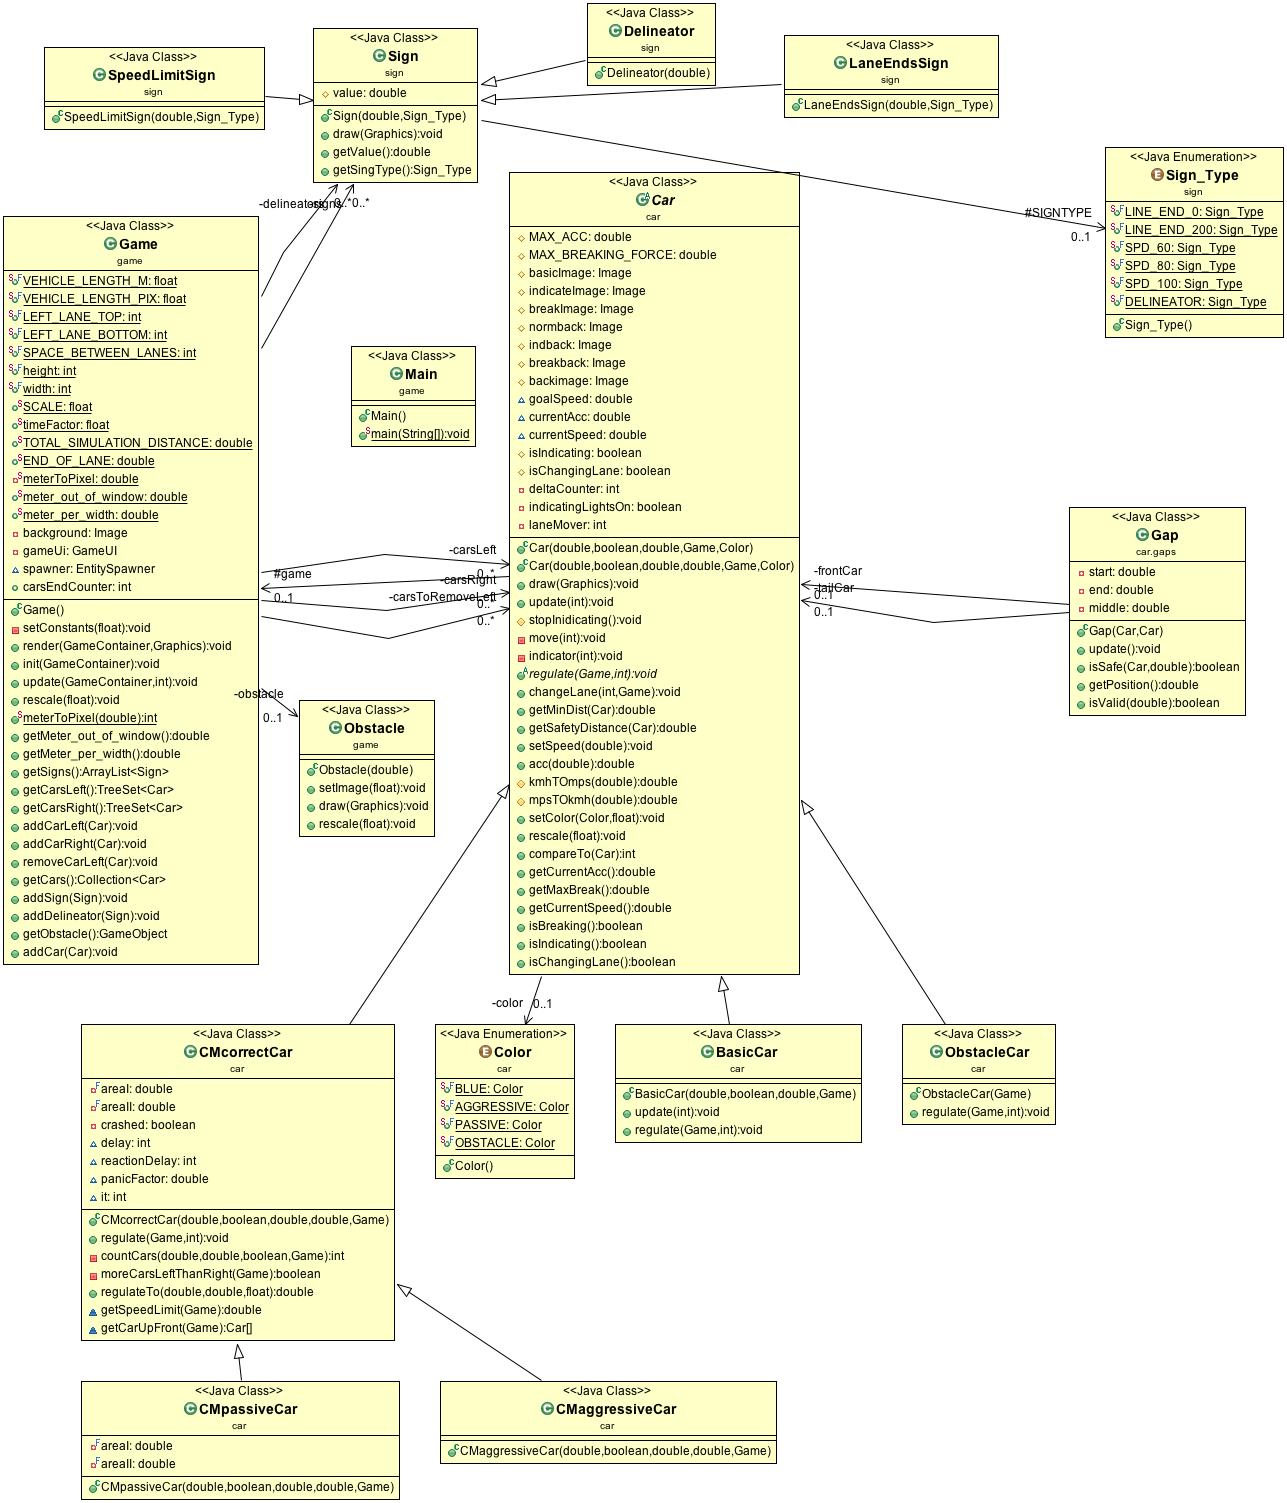
\includegraphics[width=\linewidth]{C:/Users/Christian/Desktop/PrCE/Git_Ordner/pkce/doc/tex/images/classuml}
	\caption{UML-Klassendiagramm}
	\label{fig:classuml}
\end{figure}

\begin{figure}
	
	\begin{subfigure}{0.5\linewidth}
		\centering
		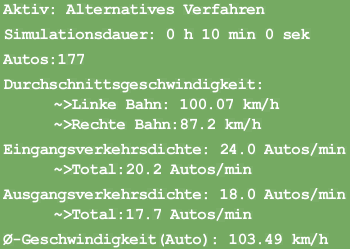
\includegraphics[width=\linewidth]{C:/Users/Christian/Desktop/PrCE/Git_Ordner/pkce/doc/tex/images/7-13_Altern_VD02}
		\caption*{}
		\label{fig:7-13alternvd02}
	\end{subfigure}
	\begin{subfigure}{0.5\linewidth}
		\centering
		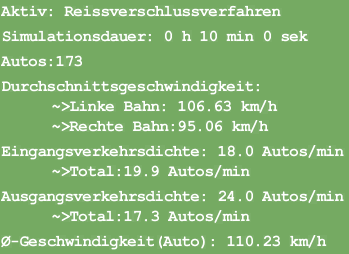
\includegraphics[width=\linewidth]{C:/Users/Christian/Desktop/PrCE/Git_Ordner/pkce/doc/tex/images/7-13_Reiss_VD02}
		\caption*{}
		\label{fig:7-13reissvd02}
	\end{subfigure}
	\begin{subfigure}{0.5\linewidth}
		\centering
		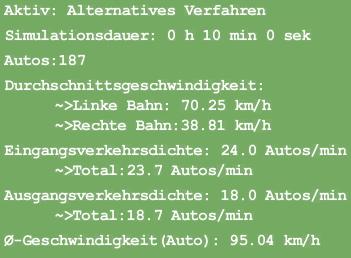
\includegraphics[width=\linewidth]{C:/Users/Christian/Desktop/PrCE/Git_Ordner/pkce/doc/tex/images/7-13_Altern_VD025}
		\caption*{}
		\label{fig:7-13alternvd025}
	\end{subfigure}
	\begin{subfigure}{0.5\linewidth}
		\centering
		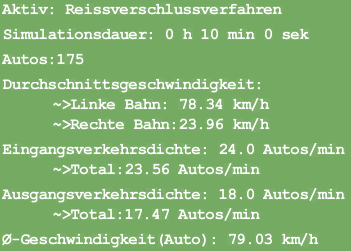
\includegraphics[width=\linewidth]{C:/Users/Christian/Desktop/PrCE/Git_Ordner/pkce/doc/tex/images/7-13_Reiss_VD025}
		\caption*{}
		\label{fig:7-13reissvd025}
	\end{subfigure}
	\begin{subfigure}{0.5\linewidth}
		\centering
		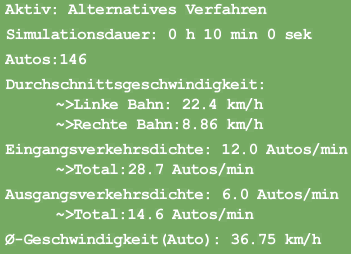
\includegraphics[width=\linewidth]{C:/Users/Christian/Desktop/PrCE/Git_Ordner/pkce/doc/tex/images/7-13_Altern_VD1}
		\caption*{}
		\label{fig:7-13alternvd1}
	\end{subfigure}
	\begin{subfigure}{0.5\linewidth}
		\centering
		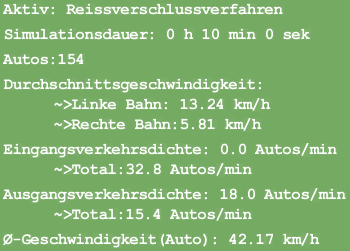
\includegraphics[width=\linewidth]{C:/Users/Christian/Desktop/PrCE/Git_Ordner/pkce/doc/tex/images/7-13_Reiss_VD1}
		\caption*{}
		\label{fig:7-13reissvd1}
	\end{subfigure}7
\caption{Simulationsdaten}
\label{simlutionsdaten}
\end{figure}